\documentclass[dvipdfmx,11pt]{beamer}

\usepackage{bxdpx-beamer}
%\usepackage{listings,jlisting}
\usepackage{tikz}
\usepackage{otf}
\usepackage{graphicx}
\usepackage{colortbl}
\usepackage{pdfpages}
\usetikzlibrary{positioning}
\usetikzlibrary{shadows}
\AtBeginDvi{\special{pdf:tounicode 90ms-RKSJ-UCS2}} 
\setbeamertemplate{navigation symbols}{} %% 右下のアイコンを消す

\renewcommand{\kanjifamilydefault}{\gtdefault}

\usetheme{Berlin}
%\usetheme{Darmstadt}

\setbeamertemplate{footline}[frame number] %% スライド下のバーを消してフレーム番号を表示
\useoutertheme{shadow}                 %% 箱に影をつける
\usefonttheme{professionalfonts}       %% 数式の文字を通常の LaTeX と同じにする

\usepackage{graphicx,xcolor}

\title{解集合プログラミングを用いた\\グラフ彩色問題の解法に関する考察}
\author{春田 穂高}
\date{2021年度番原研中間発表会\\2021年12月3日}
\institute{番原研究室}

%%%%%%%%%%%%%%%%%%%%%%%%%%%%%%%%%%%%%%%%%%%%%%%%%%%%%%%%%%%%%%%%%%%%%%%%%%%%%%%%%%%%%%%%
%%本文
%%%%%%%%%%%%%%%%%%%%%%%%%%%%%%%%%%%%%%%%%%%%%%%%%%%%%%%%%%%%%%%%%%%%%%%%%%%%%%%%%%%%%%%%

\begin{document}
\begin{frame}{}
 \titlepage
\end{frame}

%%%%%%%%%%%%%%%%%%%%%%%%%%%%%%%%%%%%%%%%%%%%%%%%%%%%%%%%%%%%%%%%%%%%%%%%%%%%%%%%%%%%%%%%

\begin{frame}{グラフ彩色問題(graph coloring)}
 \begin{block}{グラフ彩色問題の定義}
  与えられたグラフ$G=(V,E)$と色数$k$に対して,以下の制約を満たす解が存在するかを判定する問題.
  \begin{itemize}
   \item 各頂点は少なくとも1つの色で塗られる.
   \item $(u,v) \in E$である$u,v \in V$について,$u$と$v$は異なる色で塗られる.
  \end{itemize}
 \end{block}

 \begin{exampleblock}{グラフ彩色問題の例}
  \begin{columns}
   \begin{column}{0.50\textwidth}
    \centering
    %%%%%%%%%%%%%%%%%%%%%%%%%%%%%%%%%%%%%%%%%%%%%%%%%%
% 実行例(t=0) (第6章で使う)
%%%%%%%%%%%%%%%%%%%%%%%%%%%%%%%%%%%%%%%%%%%%%%%%%%

\begin{tikzpicture}[scale=0.6]

  % 設定
  \tikzset{node/.style={circle,draw=black}}
 
  \definecolor{col_r}{RGB}{230,0,18}
  %\definecolor{col_b}{RGB}{0,104,183}
  \definecolor{col_b}{RGB}{51,51,179}
  \definecolor{col_y}{RGB}{255,251,0}
  \definecolor{col_g}{RGB}{0,96,0}
 
  % 補助線
  % \draw [help lines,blue] (0,0) grid (20,6);
 
  % node %
  \node[node, fill=col_y!70] (node1){\textbf{1}};
  \node[node, fill=col_b!70, right=of node1] (node2){\textbf{2}};
  \node[node, fill=col_y!70, below=of node1] (node3){\textbf{3}};
  \node[node, fill=col_g!70, below=of node2] (node4){\textbf{4}};
 
  \foreach \u / \v in {node1/node2, node2/node3, node2/node4, node3/node4}
  \draw (\u) -- (\v);
 \end{tikzpicture}
 
 %%%%%%%%%%%%%%%%%%%%%%%%%%%%%%%%%%%%%%%%%%%%%%%%%%%%%%%%%%
 %%% Local Variables:
 %%% mode: japanese-latex
 %%% TeX-master: paper.tex
 %%% End:
 
   \end{column}
  \end{columns}
 \end{exampleblock}
\end{frame}

%%%%%%%%%%%%%%%%%%%%%%%%%%%%%%%%%%%%%%%%%%%%%%%%%%%%%%%%%%%%%%%%%%%%%%%%%%%%%%%%%%%%%%%%

\begin{frame}{解集合プログラミング(Answer Set Programing)}
 \begin{itemize}
  \item ASP言語は一階論理に基づいた知識表現言語の一種である.
  \item ASPシステムは,安定モデル意味論~[Gelfond and Lifschitz '88]
        に基づく解集合を計算するシステムである.
  \item 近年,SAT技術を利用した高速なASPシステムが開発され,
        様々な分野への実用的応用が急速に拡大している.
 \end{itemize}
 \begin{alertblock}{グラフ彩色問題に対してASPを用いる利点}
  \begin{itemize}
   \item ASP言語の高い表現力により,記号上の制約を簡潔に記述できる.
   \item 充足不能コアなどのSAT技術を利用した最適値探索が可能.
  \end{itemize}
 \end{alertblock}
\end{frame}

%%%%%%%%%%%%%%%%%%%%%%%%%%%%%%%%%%%%%%%%%%%%%%%%%%%%%%%%%%%%%%%%%%%%%%%%%%%%%%%%%%%%%%%%

\begin{frame}{研究目的}
 \begin{alertblock}{目的}
  グラフ彩色問題に対して,ASPを利用して符号化を提案し,実験,評価する.
 \end{alertblock}

 \begin{block}{研究内容}
  \begin{itemize}
   \item McGregorグラフにおいて4種の彩色問題に対する4つの符号化の実装.
         \begin{itemize}
          \item グラフ彩色問題を解く符号化
          \item ある色の彩色数を最大化,最小化した際の符号化
          \item 多色で彩色される頂点数を最大化した際の符号化
         \end{itemize}
   \item 各符号化についてMcGregorグラフで実験.
  \end{itemize}
 \end{block}
\end{frame}

%%%%%%%%%%%%%%%%%%%%%%%%%%%%%%%%%%%%%%%%%%%%%%%%%%%%%%%%%%%%%%%%%%%%%%%%%%%%%%%%%%%%%%%%

\begin{frame}{McGregorグラフ}
 \begin{block}{McGregorグラフ}
  \begin{itemize}
   \item オーダーnを決定することで決定されるグラフ.
   \item 頂点数$N=n*(n+1)$個,辺数$3N-6$個からなるグラフ.
   \item 頂点は$(j,k)(0\leq j \leq n) (0 \leq k < n)$で表される.
  \end{itemize}
 \end{block}
 \begin{exampleblock}{オーダー$n=10$のMcGregorグラフ}
    \centering
    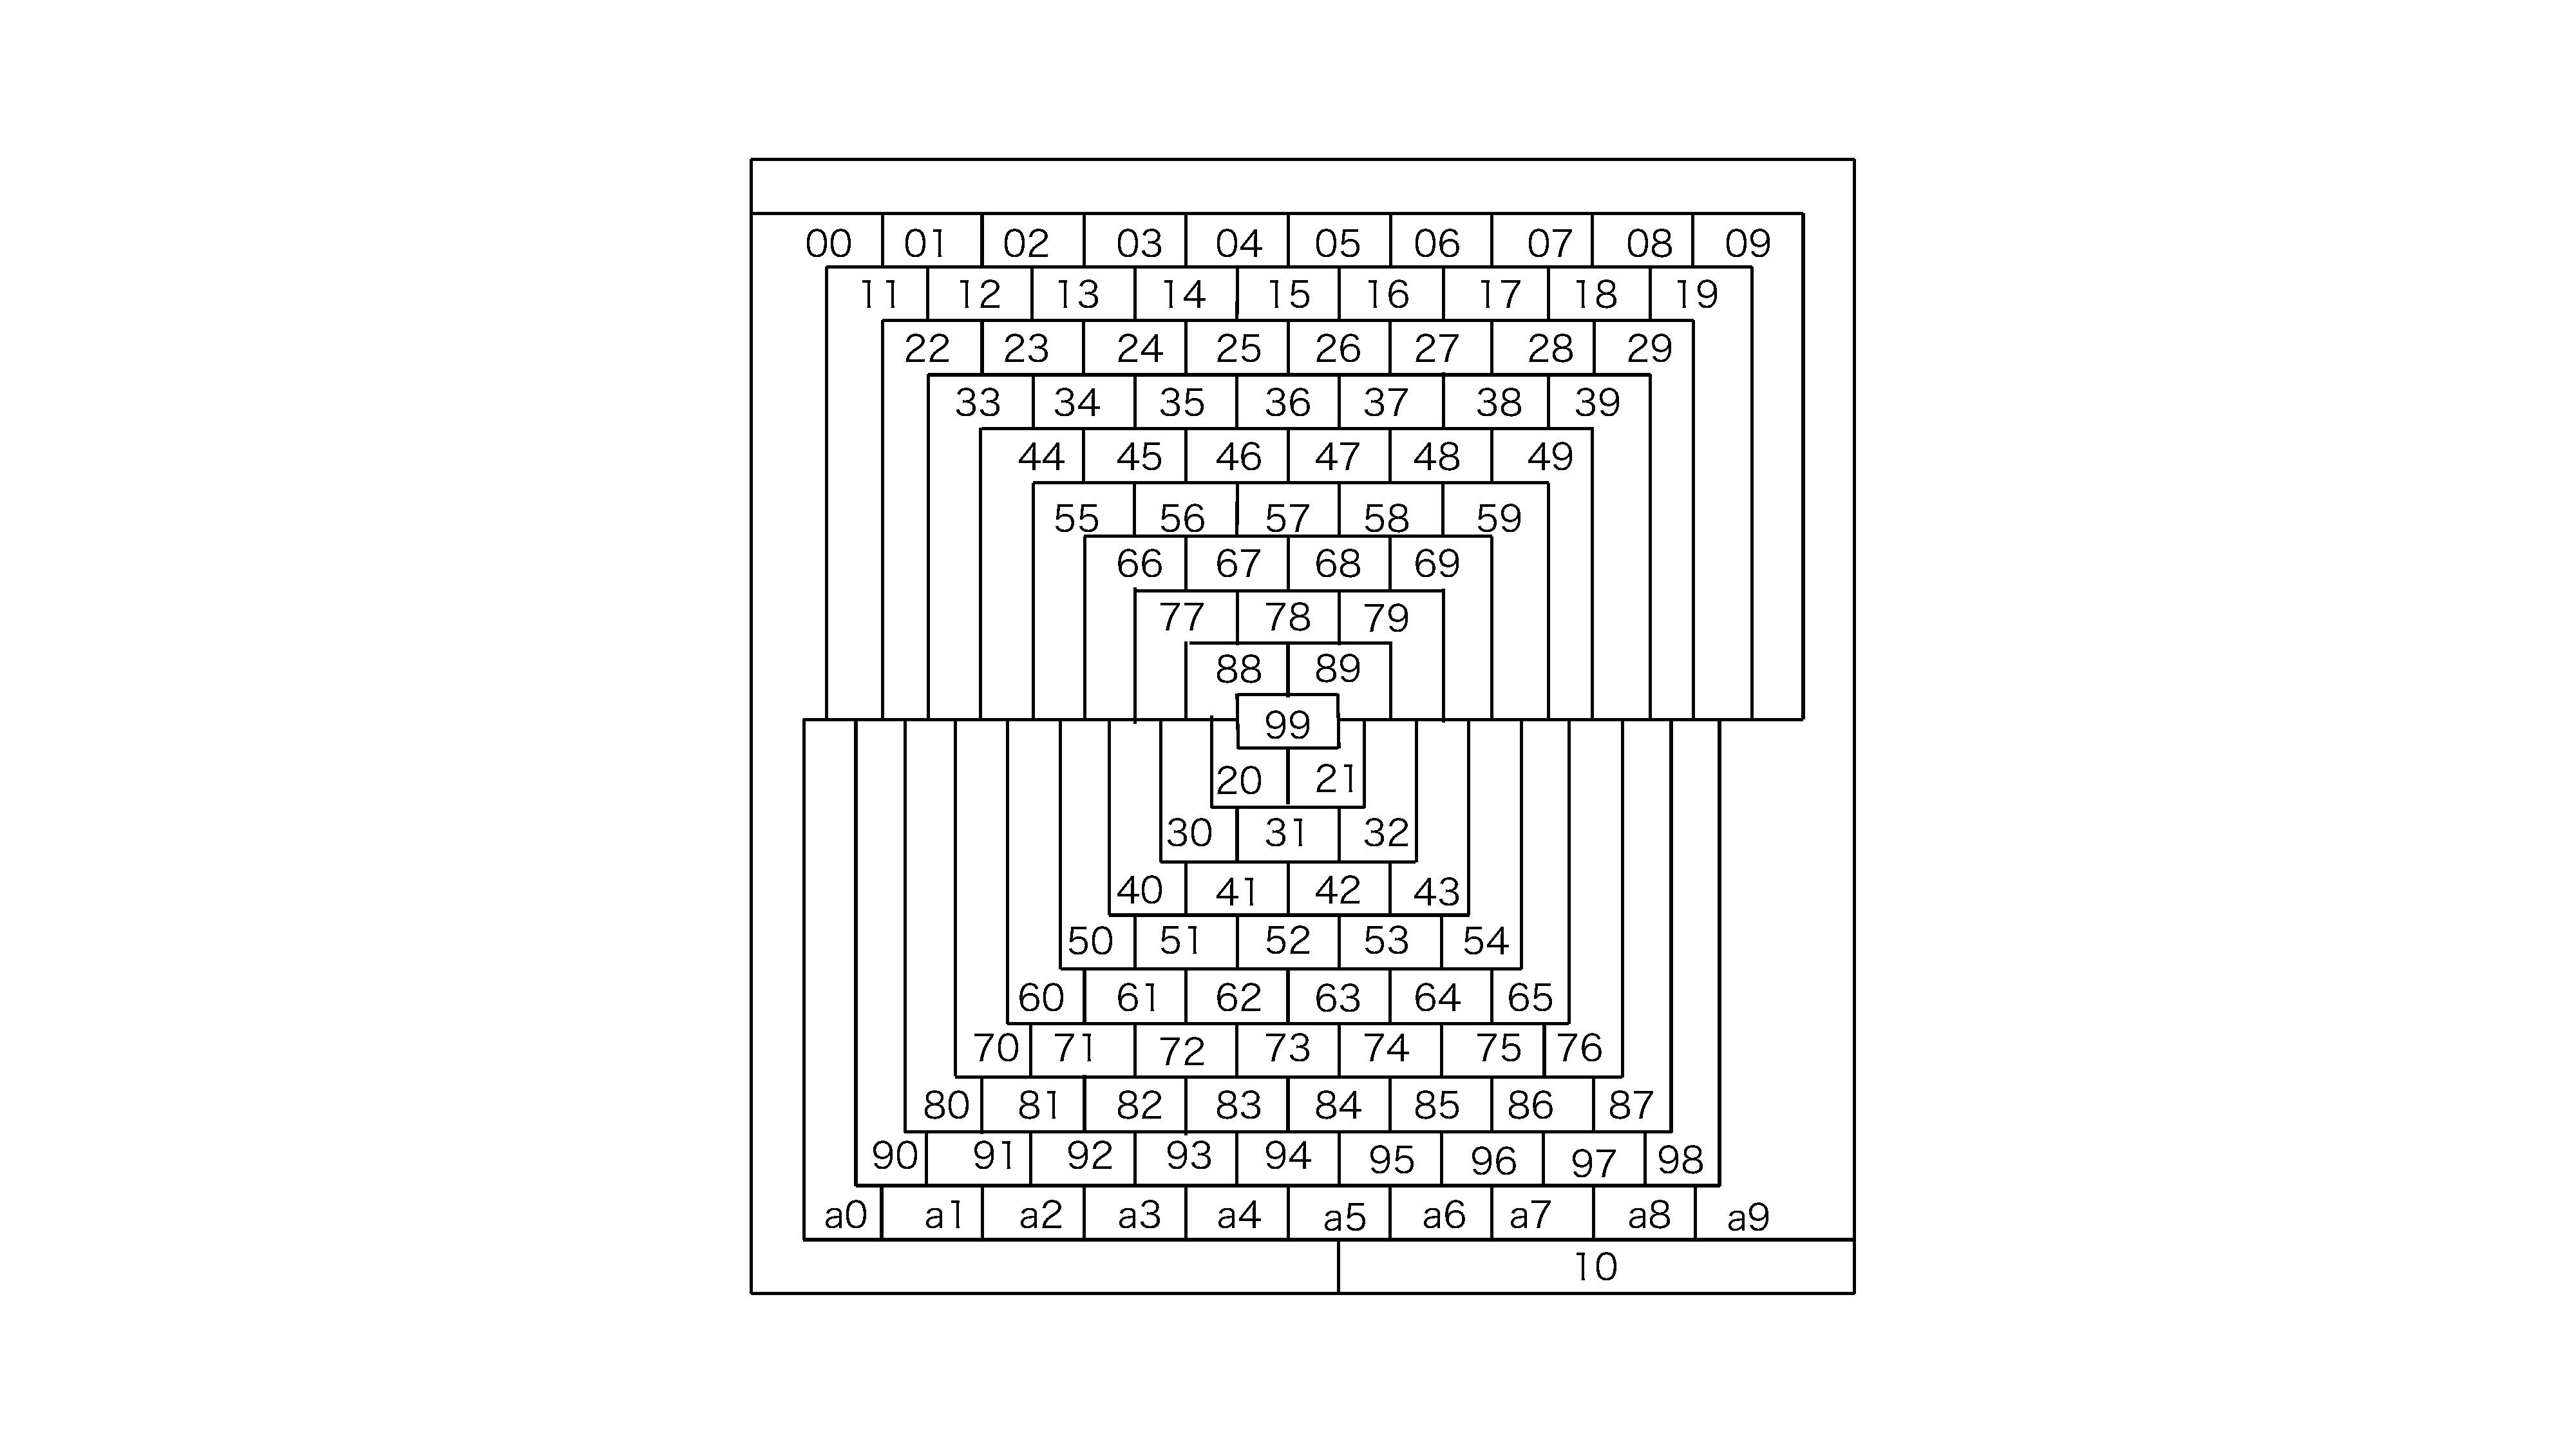
\includegraphics[keepaspectratio, scale=0.15]{graph2.pdf}
 \end{exampleblock}
 
\end{frame}

%%%%%%%%%%%%%%%%%%%%%%%%%%%%%%%%%%%%%%%%%%%%%%%%%%%%%%%%%%%%%%%%%%%%%%%%%%%%%%%%%%%%%%%%

\begin{frame}{ASP符号化(1/2)}
 \begin{block}{グラフ彩色問題を解く符号化}
  \begin{itemize}
   \item 頂点$X$について,色$K$で彩色する\structure{$color(X,K)$}を生成する.
   \item 隣接する頂点について,同じ色で彩色しない制約を導入する.
  \end{itemize}
  この符号化を\structure{color}とする.
 \end{block}
 \begin{block}{多色で塗ることのできる頂点数を最大化した際の符号化}
  \begin{itemize}
   \item 頂点$X$について,色$K$で彩色する\structure{$color(X,K)$}を生成する.
   \item 隣接する頂点について,同じ色で彩色しない制約を導入する.
   \item ある頂点$X$について,複数の色で塗られている場合,
         \structure{$mult(X)$}を生成する.
   \item \structure{$mult(X)$}について,その頂点$X$の数を\alert{最大化}する制約を導入する.
  \end{itemize}
  この符号化を\structure{mult}とする.
 \end{block}
\end{frame}

%%%%%%%%%%%%%%%%%%%%%%%%%%%%%%%%%%%%%%%%%%%%%%%%%%%%%%%%%%%%%%%%%%%%%%%%%%%%%%%%%%%%%%%%

\begin{frame}{ASP符号化(2/2)}
 \begin{block}{ある色の彩色数を最小化した際の符号化}
  \begin{itemize}
   \item ある色に対して彩色数を\alert{最小化}する制約を導入する.
  \end{itemize}
   符号化\structure{color}にこの制約を追加した符号化を\structure{minimize}とする.
 \end{block}
 \begin{block}{ある色の彩色数を最大化した際の符号化}
  \begin{itemize}
   \item ある色に対して彩色数を\alert{最大化}する制約を導入する.
  \end{itemize}
   符号化\structure{color}にこの制約を追加した符号化を\structure{maxmize}とする.
 \end{block}
\end{frame}

%%%%%%%%%%%%%%%%%%%%%%%%%%%%%%%%%%%%%%%%%%%%%%%%%%%%%%%%%%%%%%%%%%%%%%%%%%%%%%%%%%%%%%%%

\begin{frame}{実験内容(1/3)}
 \begin{block}{color}
  \begin{itemize}
   \item \structure{使用問題}: 138問 \\
         \textit{The Art of Computer Programming}で解説されている \\
         McGregorグラフの定義に基づいて作成したオーダー$3 \leq n \leq 140$のグラフ
   \item \structure{色数}: 4色
   \item \structure{ASPシステム}: \textit{clingo-5.5.0}
         \begin{itemize}
          \item \structure{オプション}: \textit{trendy}
         \end{itemize}
   \item \structure{制限時間}: 1800秒/問
   \item \structure{実験環境}:Mac mini(3.2GHz 64GB)
  \end{itemize}
 \end{block}
 \begin{alertblock}{}
  結果,138問中オーダー$3 \leq n \leq 138$のグラフにおいて4色での解が見つかった.
 \end{alertblock}
\end{frame}

%%%%%%%%%%%%%%%%%%%%%%%%%%%%%%%%%%%%%%%%%%%%%%%%%%%%%%%%%%%%%%%%%%%%%%%%%%%%%%%%%%%%%%%%

\begin{frame}{実験内容(2/3)}
 \begin{block}{minimize,maxmize}
  \begin{itemize}
   \item \structure{使用問題}: 18問 \\
         \textit{The Art of Computer Programming}で解説されている \\
         McGregorグラフの定義に基づいて作成したオーダー$3 \leq n \leq 20$のグラフ
   \item \structure{色数}: 4色
   \item \structure{ASPシステム}: \textit{clingo-5.5.0}
         \begin{itemize}
          \item \structure{strategy}: \textit{BB, USC}
          \item \structure{オプション}: \textit{trendy}
         \end{itemize}
   \item \structure{制限時間}: 1800秒/問
   \item \structure{実験環境}:Mac mini(3.2GHz 64GB)
  \end{itemize}
 \end{block}
\end{frame}

%%%%%%%%%%%%%%%%%%%%%%%%%%%%%%%%%%%%%%%%%%%%%%%%%%%%%%%%%%%%%%%%%%%%%%%%%%%%%%%%%%%%%%%%

\begin{frame}{実験内容(3/3)}
 \begin{block}{mult}
  \begin{itemize}
   \item \structure{使用問題}: 13問 \\
         \textit{The Art of Computer Programming}で解説されている \\
         McGregorグラフの定義に基づいて作成したオーダー$3 \leq n \leq 15$のグラフ
   \item \structure{色数}: 4色
   \item \structure{ASPシステム}: \textit{clingo-5.5.0}
         \begin{itemize}
          \item \structure{strategy}: \textit{BB, USC}
          \item \structure{オプション}: \textit{trendy}
         \end{itemize}
   \item \structure{制限時間}: 1800秒/問
   \item \structure{実験環境}:Mac mini(3.2GHz 64GB)
  \end{itemize}
 \end{block}
\end{frame}

%%%%%%%%%%%%%%%%%%%%%%%%%%%%%%%%%%%%%%%%%%%%%%%%%%%%%%%%%%%%%%%%%%%%%%%%%%%%%%%%%%%%%%%%

\begin{frame}{実験結果(1/3)}
 \begin{block}{minimize}
  符号化\structure{minimize}の実験結果
  \begin{itemize}
   \item BB法とUSC法の両方において以下の結果の通りになった.
         \begin{table}
          \begin{tabular}{l|r|r||l|r|r}
           \hline
           order & BB & USC & order & BB & USC \\
           \hline
           3  & \alert{2}  & \alert{2}   & 12 & \alert{9}  & \alert{9}  \\
           4  & \alert{2}  & \alert{2}   & 13 & \alert{10} & \alert{10} \\
           5  & \alert{3}  & \alert{3}   & 14 & 12         & \alert{12} \\
           6  & \alert{4}  & \alert{4}   & 15 & 13         & 49         \\
           7  & \alert{5}  & \alert{5}   & 16 & 19         & \alert{12} \\
           8  & \alert{7}  & \alert{7}   & 17 & 21         & \alert{13} \\
           9  & \alert{7}  & \alert{7}   & 18 & 19         & \alert{14} \\
           10 & \alert{7}  & \alert{7}   & 19 & 20         & 58         \\
           11 & \alert{8}  & \alert{8}   & 20 & 22         & 59         \\
           \hline
          \end{tabular}
         \end{table}
   \item USC法の結果が優れていた.
  \end{itemize}
 \end{block}
\end{frame}

%%%%%%%%%%%%%%%%%%%%%%%%%%%%%%%%%%%%%%%%%%%%%%%%%%%%%%%%%%%%%%%%%%%%%%%%%%%%%%%%%%%%%%%%

\begin{frame}{実験結果(2/3)}
 \begin{block}{maximize}
  符号化\structure{maximize}の実験結果
  \begin{itemize}
   \item BB法とUSC法の両方において以下の結果の通りになった.
         \begin{table}
          \begin{tabular}{l|r|r||l|r|r}
           \hline
           order & BB & USC & order & BB & USC \\
           \hline
           3  & \alert{4}   & \alert{4}    & 12 & 48         & \alert{50}  \\
           4  & \alert{6}   & \alert{6}    & 13 & 56         & \alert{58}  \\
           5  & \alert{10}  & \alert{10}   & 14 & 56         & \alert{68}  \\
           6  & \alert{13}  & \alert{13}   & 15 & 70         & \alert{77}  \\
           7  & \alert{17}  & \alert{17}   & 16 & 71         & \alert{88}  \\
           8  & \alert{23}  & \alert{23}   & 17 & 75         & \alert{99}  \\
           9  & 28          & \alert{28}   & 18 & 91         & \alert{111} \\
           10 & 35          & \alert{35}   & 19 & 92         & \alert{123} \\
           11 & 42          & \alert{42}   & 20 & 109        & \alert{137} \\
           \hline
          \end{tabular}
         \end{table}
   \item USC法の結果が優れていた.
  \end{itemize}
 \end{block}
\end{frame}

%%%%%%%%%%%%%%%%%%%%%%%%%%%%%%%%%%%%%%%%%%%%%%%%%%%%%%%%%%%%%%%%%%%%%%%%%%%%%%%%%%%%%%%%

\begin{frame}{実験結果(3/3)}
 \begin{block}{mult}
  符号化\structure{mult}の実験結果
  \begin{itemize}
   \item BB法とUSC法の両方において以下の結果の通りになった.
         \begin{table}
          \begin{tabular}{l|r|r||l|r|r}
           \hline
           order & BB & USC & order & BB & USC \\
           \hline
           3  & \alert{1}   & \alert{1}    & 10 & 23         & \alert{23}  \\
           4  & \alert{3}   & \alert{3}    & 11 & 27         & \alert{29}  \\
           5  & \alert{4}   & \alert{4}    & 12 & 33         & \alert{36}  \\
           6  & \alert{7}   & \alert{7}    & 13 & 38         & 15          \\
           7  & \alert{9}   & \alert{9}    & 14 & 44         & 11          \\
           8  & \alert{13}  & \alert{13}   & 15 & 49         & 20          \\
           9  & \alert{18}  & \alert{18}   \\
           \hline
          \end{tabular}
         \end{table}
   \item USC法の結果が優れていた.
  \end{itemize}
 \end{block}
\end{frame}

%%%%%%%%%%%%%%%%%%%%%%%%%%%%%%%%%%%%%%%%%%%%%%%%%%%%%%%%%%%%%%%%%%%%%%%%%%%%%%%%%%%%%%%%

\begin{frame}{まとめと今後の課題}
 \begin{block}{まとめ}
  \begin{itemize}
   \item McGregorグラフにおいて4種の彩色問題に対する4つの符号化を実装した.
         \begin{itemize}
          \item \alert{color}: グラフを彩色する符号化
          \item \alert{minimize}: ある色の彩色数を最小化する符号化
          \item \alert{maximize}: ある色の彩色数を最大化する符号化
          \item \alert{mult}: 多色で彩色される頂点を最大化する符号化
         \end{itemize}
   \item 各符号化についてMcGregorグラフで実験.
         \begin{itemize}
          \item \structure{minimize}, \structure{maximize}, \structure{mult}の最適化問題では \\
                USC法がより大きいオーダーで最適値を示した.
         \end{itemize}
  \end{itemize}
 \end{block}

 \begin{alertblock}{今後の課題}
  \begin{itemize}
   \item より大きいサイズのグラフでの実験.
   \item より長い制限時間内での実験.
   \item McGregorグラフ以外のグラフに対しての実験.
  \end{itemize}
 \end{alertblock}
 
\end{frame}

%%%%%%%%%%%%%%%%%%%%%%%%%%%%%%%%%%%%%%%%%%%%%%%%%%%%%%%%%%%%%%%%%%%%%%%%%%%%%%%%%%%%%%%%

\begin{frame}
 補足
\end{frame}


%%%%%%%%%%%%%%%%%%%%%%%%%%%%%%%%%%%%%%%%%%%%%%%%%%%%%%%%%%%%%%%%%%%%%%%%%%%%%%%%%%%%%%%%

\begin{frame}{実験結果}
 \begin{block}{minimize}
  符号化\structure{minimize}の実験結果
  \begin{itemize}
   \item BB法とUSC法の両方において以下の結果の通りになった.
         \centering
         {\tiny \begin{tabular}[l]{l|r|r|r||l|r|r|r}
          \hline
          order & optimization & BB & USC & order & optmization & BB & USC \\
          \hline
          3  & 2 & \alert{0.002}  & \alert{0.002}   & 12 & 9  & 166.314  & \alert{0.351}  \\
          4  & 2 & \alert{0.003}  & \alert{0.003}   & 13 & 10 & 1172.519 & \alert{0.288} \\
          5  & 3 & 0.013  & \alert{0.003}   & 14 & 12 & -      & \alert{132.131} \\
          6  & 4 & 0.049  & \alert{0.006}   & 15 & -  & -        & -        \\
          7  & 5 & \alert{0.197}  & 0.024   & 16 & 12 & -       & \alert{1.930} \\
          8  & 7 & \alert{0.941}  & 0.095   & 17 & 13 & -        & \alert{56.514} \\
          9  & 7 & 1.316  & \alert{0.025}   & 18 & 14 & -        & \alert{74.041} \\
          10 & 7 & 1.436  & \alert{0.023}   & 19 & -  & -       & -        \\
          11 & 8 & 14.002  & \alert{0.185}   & 20 & -  & -    & -         \\
          \hline
         \end{tabular}}
  \end{itemize}
 \end{block}
\end{frame}

%%%%%%%%%%%%%%%%%%%%%%%%%%%%%%%%%%%%%%%%%%%%%%%%%%%%%%%%%%%%%%%%%%%%%%%%%%%%%%%%%%%%%%%%

\begin{frame}{実験結果}
 \begin{block}{maximize}
  符号化\structure{maximize}の実験結果
  \begin{itemize}
   \item BB法とUSC法の両方において以下の結果の通りになった.
         \centering
         {\tiny \begin{tabular}[l]{l|r|r|r||l|r|r|r}
 \hline
 order & optimization & BB & USC & order & optmization & BB & USC \\
 \hline
 3  & 4 & \alert{0.002}  & \alert{0.002}   & 12 & 50  & -  & \alert{0.077}  \\
 4  & 6 & \alert{0.003}  & \alert{0.003}   & 13 & 58 & - & \alert{0.043} \\
 5  & 10 & 0.005  & \alert{0.003}   & 14 & 68 & -      & \alert{0.099} \\
 6  & 13 & \alert{0.003}  & 0.005   & 15 & 77  & -        & \alert{1.433}       \\
 7  & 17 & 1.041  & \alert{0.007}   & 16 & 88 & -       & \alert{0.555} \\
 8  & 23 & 69.767  & \alert{0.009}   & 17 & 99 & -        & \alert{1.046} \\
 9  & 28 & -  & \alert{0.016}   & 18 & 111 & -        & \alert{0.287} \\
 10 & 35 & -  & \alert{0.017}   & 19 & 123  & -       & \alert{1.954}       \\
 11 & 42 & -  & \alert{0.026}   & 20 & 137  & -    & \alert{1.083}       \\
 \hline
\end{tabular}}
  \end{itemize}
 \end{block}
\end{frame}

%%%%%%%%%%%%%%%%%%%%%%%%%%%%%%%%%%%%%%%%%%%%%%%%%%%%%%%%%%%%%%%%%%%%%%%%%%%%%%%%%%%%%%%%

\begin{frame}{実験結果}
 \begin{block}{mult}
  符号化\structure{mult}の実験結果
  \begin{itemize}
   \item BB法とUSC法の両方において以下の結果の通りになった.
         \centering
         {\tiny \begin{tabular}[l]{l|r|r|r||l|r|r|r}
 \hline
 order & optimization & BB & USC & order & optmization & BB & USC \\
 \hline
 3  & 1 & \alert{0.003}  & 0.004   & 12 & 36  & -  & \alert{196.726}  \\
 4  & 3 & 0.016  & \alert{0.009}   & 13 & - & - & - \\
 5  & 4 & 0.099  & \alert{0.084}   & 14 & - & -      & - \\
 6  & 7 & \alert{0.291}  & 0.829   & 15 & -  & -        & -     \\
 7  & 9 & \alert{0.812}  & 7.530   & 16 & - & -       & - \\
 8  & 13 & \alert{3.483}  & 15.040  & 17 & - & -        & - \\
 9  & 18 & 203.468  &  \alert{39.851}   & 18 & - & -        & - \\
 10 & 23 & -  & \alert{126.909}   & 19 & -  & -       & -       \\
 11 & 29 & -  & \alert{1006.760}   & 20 & -  & -    & -       \\
 \hline
\end{tabular}}
  \end{itemize}
 \end{block}
\end{frame}

%%%%%%%%%%%%%%%%%%%%%%%%%%%%%%%%%%%%%%%%%%%%%%%%%%%%%%%%%%%%%%%%%%%%%%%%%%%%%%%%%%%%%%%%
\end{document}
